\documentclass[conference,10pt]{IEEEtran}
\IEEEoverridecommandlockouts
% The preceding line is only needed to identify funding in the first footnote. If that is unneeded, please comment it out.
\usepackage{cite}
\usepackage{ctex}
\usepackage{amsmath,amssymb,amsfonts}
\usepackage{algorithmic}
\usepackage{graphicx}
\usepackage{textcomp}
\usepackage{xcolor}
\usepackage{float}
\usepackage{subfigure}
\def\BibTeX{{\rm B\kern-.05em{\sc i\kern-.025em b}\kern-.08em
    T\kern-.1667em\lower.7ex\hbox{E}\kern-.125emX}}
\begin{document}

\title{OK-VQA: A Visual Question Answering Benchmark Requiring External Knowledge}

\author{\IEEEauthorblockN{
		% 1\textsuperscript{st} 
		承子杰}
	\IEEEauthorblockA{\textit{dept. AMSS(数学与系统科学研究院)} \\
		\textit{of CAS (中国科学院)}\\
		chengzijie22@mails.ucas.ac.cn\\
		202228000243001}}
\maketitle

\section{主要内容}
文章作者认为VQA应该能从图像和文本的联合信息中学习推理,从而进行场景理解。然而现有的大部分VQA不需要外部知识(knowledge-based)和逻辑推理,仅局限于计数、目标检测等简单任务。因此作者提出了OK-VQA数据集,数据集中提出的问题需要结合外部知识来进行回答。此外作者提出了一种ArticleNet的方法用于结合外部知识,并选择了一系列VQA模型与其结合,给出了它们在OK-VQA数据集上的BenchMark用作后续研究作为基准。
\section{OK-VQA数据集的建立}
\subsection{数据来源}
作者对VQA数据集中10000个问题进行Age Annotation,发现其 78\% 的问题可以由10岁以下的儿童回答,因此作者认为 VQA数据集大部分问题不需要背景知识。因此 OK-VQA 的图像数据来源于MS COCO的随机图像,选取其中 80K 张图片作为训练数据集,40K张图片作为验证数据集,场景覆盖了COCO数据中365个场景中的350个。
\subsection{数据标注}
作者将120K张图片在Amazon的MTurk平台上进行外包,经历了两轮标注。在第一轮标注中,作者要求标注者对于每一张图片提出一个问题,要求该问题与图像相关,且需要依赖一定的外部知识。在第二轮标注中,要求 5 个标注者分别对第一轮标注提出的问题进行回答,以确保提出的问题具有一定价值。最后再进行一次人工筛选,筛出 34,921 个问题。

考虑到数据集存在偏差,作者将第二轮回答中出现5个答案一致的问题和5个答案均不一致的问题进行删除,最终留下了 14,055 个问题。其中,9009 个作为训练问题,5046 个作为训练问题。图\ref{sample}展示了数据集中的一些示例样本。
\begin{figure}
	\centering
	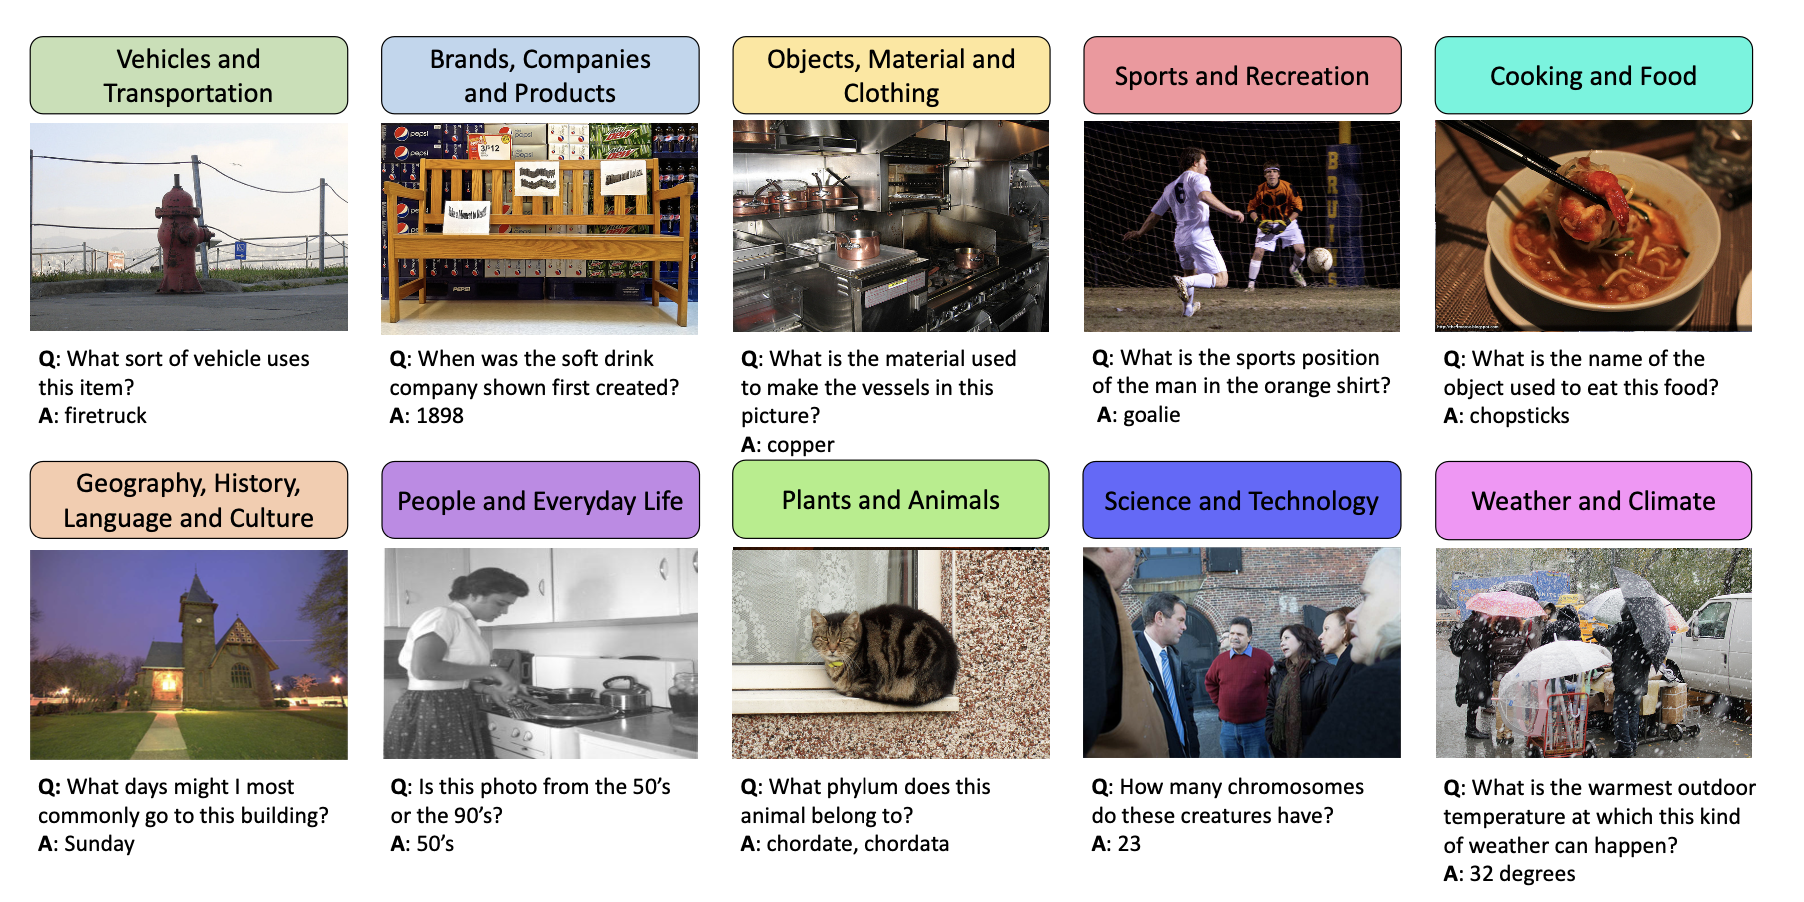
\includegraphics[scale=0.3]{figure/sample.png}
	\caption{OK-VQA 数据集样本示例}
	\label{sample}
\end{figure}
\subsection{数据结构}
作者对数据集做了知识类别划分(Knowledge Category)。他们将问题分为10+1类,类别涵盖了车辆和交通(Vehicles and Transportation)、商标公司和产品(Brands,Companies and Products)、材料和衣服(Objects, Materials and Clothing)、运动和娱乐(Sports and Recreation)、烹饪和食品(Cooking and Food)、历史文化与地理(Geography, History, Language and Culture)、日常生活与动植物(People and Everyday Life, Plants and Animals)、科学与技术(Science and Technology)、气候环境(Weather and Climate)10个类别和一个其他(Other)类别,各类别在数据集中的分布情况见图\ref{category}。

此外,作者还进行了数据集问题统计(Question Statistics)。经过作者统计,在提出的140,55个问题中有12,591种问题类别(即非重复问题数量),问题题干涉及了 7178 个单词。除此之外,作者还统计了10+1个知识类别中相对频率最高的问题单词和答案单词,统计结果见图\ref{statistics}。通过观察,我们发现问题单词与答案单词间具有很高的关联性,具有一定的上下位关系。
\begin{figure}
	\centering
	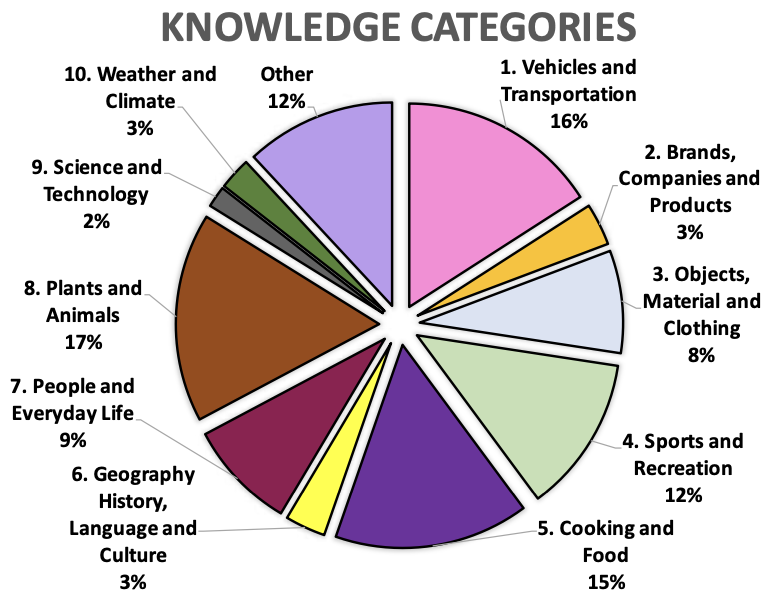
\includegraphics[scale=0.35]{figure/category.png}
	\caption{各类别占比}
	\label{category}
\end{figure}
\begin{figure}
	\centering
	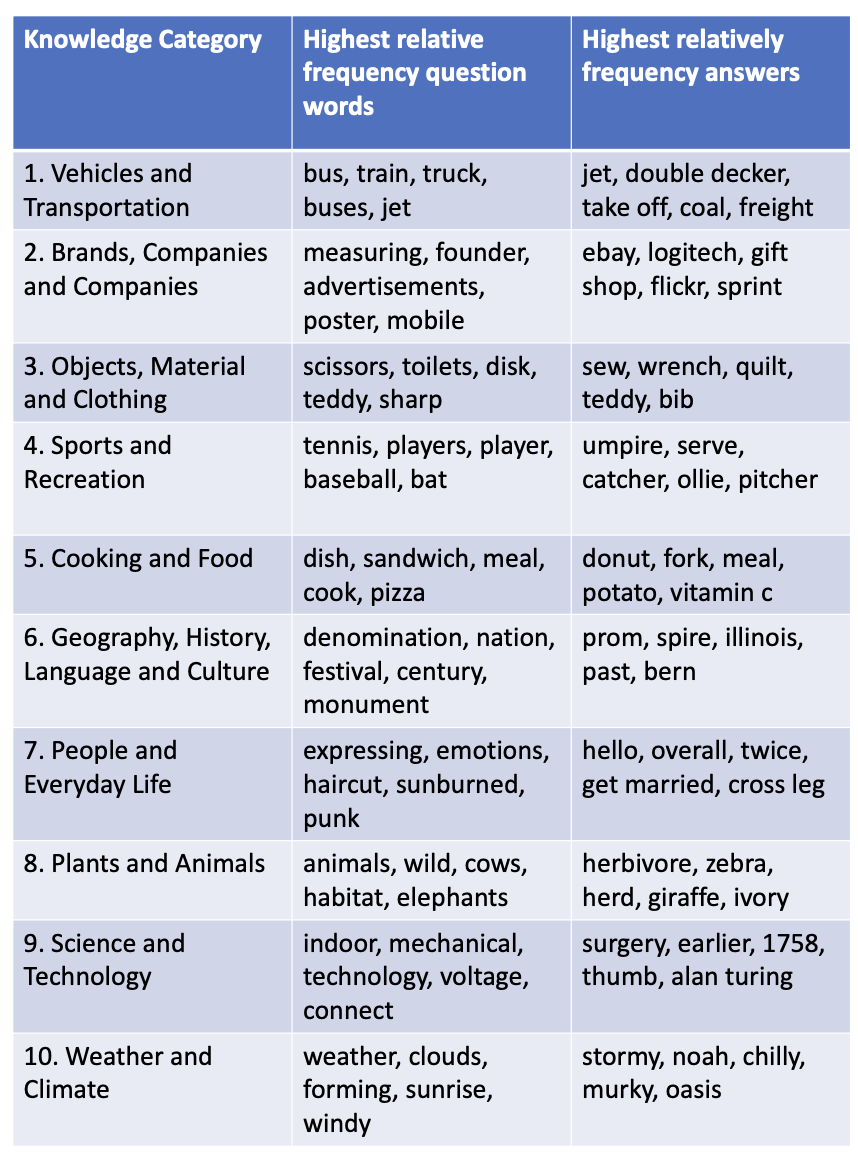
\includegraphics[scale=0.33]{figure/statistics.png}
	\caption{各类别高频问题答案单词}
	\label{statistics}
\end{figure}
\section{数据集基准(BenchMark)}

\subsection{ArticleNet}
作者提出了名为ArticleNet的框架,使得可以通过Wikipedia的API进行检索外部相关文章,以此获得非结构化外部知识。其主要框架(图\ref{ArticleNet})可以分为三步:
\begin{figure}
	\centering
	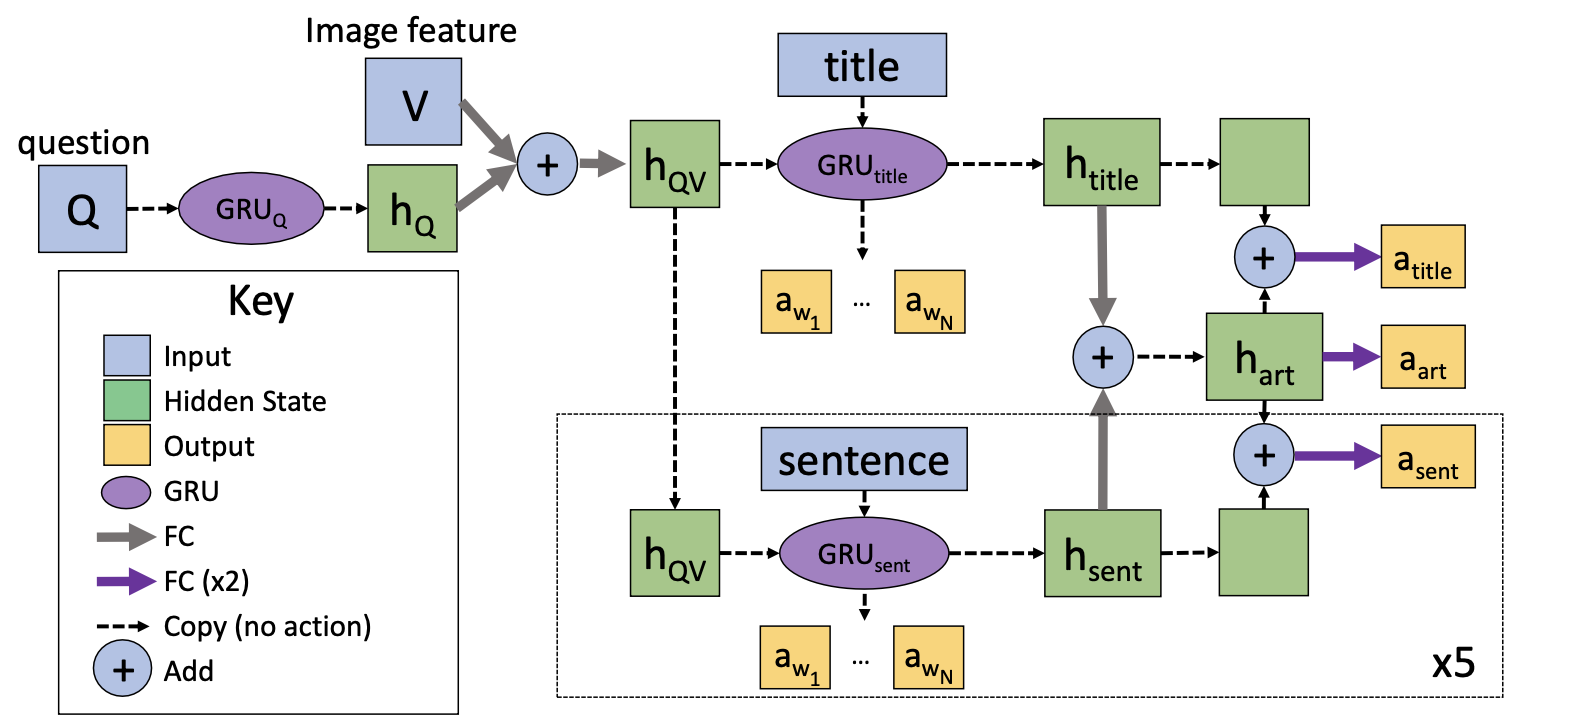
\includegraphics[scale=0.28]{figure/ArticleNet.png}
	\caption{ArticleNet 基本框架}
	\label{ArticleNet}
\end{figure}
\begin{enumerate}
	\item 对训练数据提供的图片使用图像和场景分类器识别图像特征单词,并与其问题单词结合组成所有可能的查询(query);
	\item 使用Wikipedia提供的API对每一个查询进行检索,并保留检索结果的第一篇文章。
	\item 对每个查询检索的文章,根据查询词在句子中出现的频率,选择整篇文章中最符合的句子,从而用句子来代替整篇文章的查询结果。
\end{enumerate}
ArticleNet也可以与其他VQA方法相结合,作者提供的结合方法是将查询结果句子的隐藏层表示与具体VQA模型中某一层的输出向量进行向量拼接。根据作者提供的各具体模型在OK-VQA数据上的表现(图\ref{label}),考虑到ArticleNet是基于互联网数据,且查询结合外部知识方法略显简单粗糙,单独使用ArticleNet似乎效果并不理想。但是其与MUTAN和BAN等方法结合,却有显著的效果提升。
\begin{figure}[H]
	\centering
	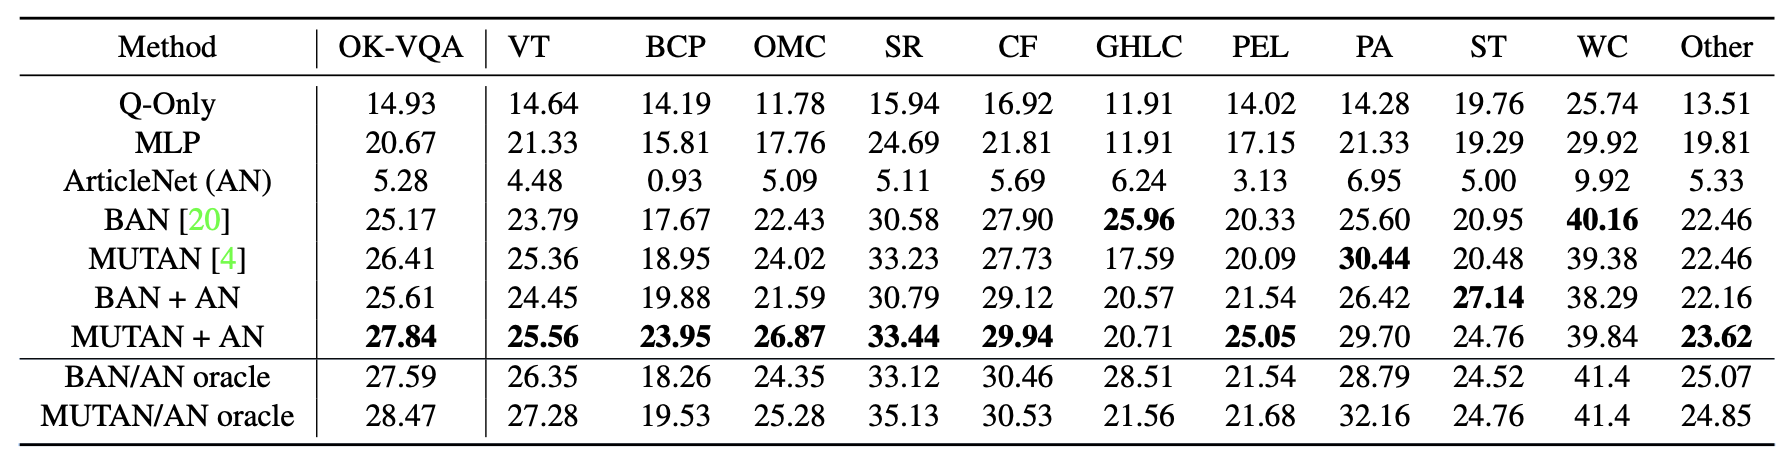
\includegraphics[scale=0.3]{figure/benchmark.png}
	\caption{BenchMark on OK-VQA}
	\label{benchmark}
\end{figure}
此外,分析BenchMark的结果,我们发现这些方法在OK-VQA数据集上的结果均大幅低于在标准VQA数据集上的结果。由此可见,对于基于外部知识的VQA任务并没有一个有效的模型,基于此类问题的研究还有很大的空间进行探索。

\subsection{视觉特征简化(Visual feature ablation)}
作者还对MUTAN做了一个简单的视觉特征简化实验,观测不同的视觉特征提取器在OK-VQA数据集上的结果变化。作者分别采用了ResNet152、ResNet50、ResNet18和Q-Only分别进行实验,结果如下:
\begin{figure}[H]
	\centering
	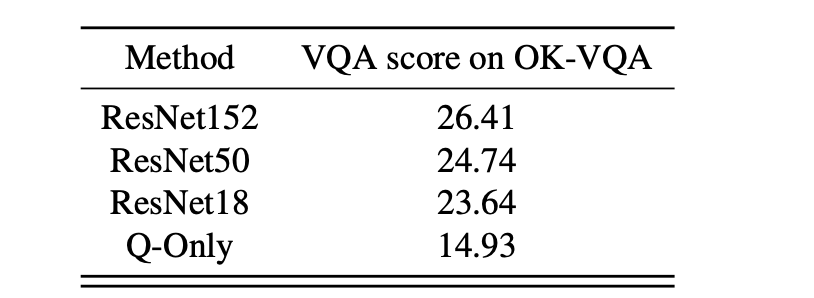
\includegraphics[scale=0.4]{figure/Visualfeature.png}
	\caption{Visual feature Ablation}
	\label{visual}
\end{figure}
通过实验结果可以发现,基本还是遵循越深的视觉特征提取器可以在OK-VQA上获得越好的结果。
\subsection{尺度简化(Scale ablation)}
最后,作者还进行了一个简单的尺度简化实验。通过对数据集中不同训练数据量进行训练,获得在测试数据集上的打分,结果如下所示
\begin{figure}[H]
	\centering
	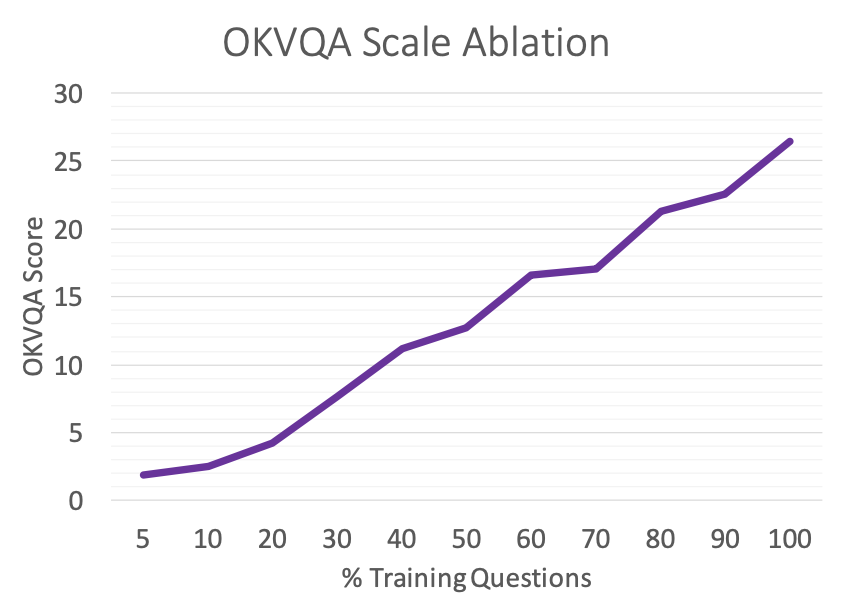
\includegraphics[scale=0.4]{figure/Scale.png}
	\caption{Scale Ablation}
	\label{scale}
\end{figure}
不难发现,数据量的提升可以获得更好的训练结果。通过视觉特征简化实验和尺度简化实验,我们可以初步判断OK-VQA是有价值的数据集。
\section{总结}
本篇文章的主要贡献主要有以下几点:
\begin{itemize}
	\item 提出了基于外部知识的VQA任务;
	\item 构建了基于外部知识的VQA数据集OK-VQA,并提供了该任务和数据集的BenchMark
	\item 提出了ArticleNet框架,为该问题的解决提供了一种思路。
	\item 通过流行VQA模型在OK-VQA上的结果指明,基于外部知识的VQA任务没有一个有效模型。该问题具有很大的挑战和研究空间。
\end{itemize}
\section*{References}
\begin{thebibliography}{00}
\bibitem{b1} Marino K, Rastegari M, Farhadi A, et al. Ok-vqa: A visual question answering benchmark requiring external knowledge[C]//Proceedings of the IEEE/cvf conference on computer vision and pattern recognition. 2019: 3195-3204.
\end{thebibliography}
\end{document}
